\section{Holomorphic Functions}
In this section we study holomorphic functions. We shall not give definitions of complex numbers in detail. Instead, we mention some basic properties of complex numbers. Throughout the book we shall use $\mathbb{C}$ to denote the field of complex numbers, $|z|$ the length of the complex number $z$.
\subsection{Definition of Holomorphic Functions}
We first mention an important inequality of complex numbers.
\begin{theorem}\label{Thm1.1.1}
Suppose $z,w\in\mathbb{C}$, then $|z+w|\le |z|+|w|$.
\end{theorem}
\begin{proof}
We first show that $\Re(zw)=\Bar{z}w+z\Bar{w}$. Suppose $z=a+b\mathrm{i}$, $w=c+d\mathrm{i}$, then 
$$
\begin{aligned}
\Re \left( z\bar{w} \right)& =\Re \left( \left( a+b\mathrm{i} \right) \left( c-d\mathrm{i} \right) \right) 
\\
&=\Re \left( ac+bd+\left( -ad+bc \right) \mathrm{i} \right) =ac+bd
\\
&=\frac{1}{2}\left[ \left( a+b\mathrm{i} \right) \left( c-d\mathrm{i} \right) +\left( c+d\mathrm{i} \right) \left( a-b\mathrm{i} \right) \right] 
\\
&=\frac{1}{2}\left( z\bar{w}+\bar{z}w \right) .
\end{aligned}
$$
Now use the inequality $\Re z\le|z|$ for all $z\in\mathbb{C}$ to obtain 
$$
\begin{aligned}
\left| z+w \right|^2&=\left( z+w \right) \left( \bar{z}+\bar{w} \right) =z\bar{z}+z\bar{w}+\bar{z}w+w\bar{w}=z^2+2\Re \left( z\bar{w} \right) +w^2
\\
&\le z^2+2\left| z\bar{w} \right|+w^2=z^2+2\left| z \right|\cdot \left| \bar{w} \right|+w^2=\left( \left| z \right|+\left| w \right| \right) ^2,
\end{aligned}
$$
which finished the proof.
\end{proof}
By Theorem \ref{Thm1.1.1} we have $\left| a_1z_1+a_2z_2+\cdots +a_nz_n \right|\le \left| a_1 \right|\cdot \left| z_1 \right|+\left| a_2 \right|\cdot \left| z_2 \right|+\cdots +\left| a_n \right|\cdot \left| z_n \right|$.\par
Since we may identify $\mathbb{C}=\mathbb{R}^2$, certain properties to $\mathbb{R}^2$ applies to $\mathbb{C}$. For instance, we may define the following convergence of a sequence of complex numbers: 
\begin{definition}
Let $\{z_n\}_{n=1}^\infty\subset\mathbb{C}$. Then the sequence $\{z_n\}$ is said to be \textbf{convergent to $z$} provided 
$$
\lim_{n\to\infty}|z_n-z|=0.
$$
\end{definition}
We have the following \textbf{Cauchy's criterion}.
\begin{theorem}
The complex sequence $\{z_n\}_{n=1}^\infty$ converges if and only if for any real number $\varepsilon>0$, there exists a natural number $n_0(\varepsilon)$ such that for all $n,m>n_0(\varepsilon)$, we have $|z_n-z_m|<\varepsilon$.
\end{theorem}
\begin{proof}
Suppose $\{z_n\}$ converges. Then for any $\varepsilon>0$, there exists some natural number $N$ such that $|z_n-z|<\varepsilon/2$ for all $n>N$. Take $N=n_0(\varepsilon)$, then for all $m,n>n_0(\varepsilon)$ we have 
$$
\left| z_m-z_n \right|\le \left| z_m-z \right|+\left| z-z_n \right|<\frac{\varepsilon}{2}+\frac{\varepsilon}{2}=\varepsilon .
$$
Conversely, suppose for each $\varepsilon>0$ there exists some $n_0(\varepsilon)$ such that for all $m,n>n_0(\varepsilon)$ we have $|z_m-z_n|<\varepsilon$. Therefore 
$$
\left| \left| z_m \right|-\left| z_n \right| \right|\le \left| z_m-z_n \right|<\varepsilon ,
$$
and hence by the Cauchy's criterion of real sequences we finished the proof.
\end{proof}
We mention another result. From $z_n\to z$ we have 
$$
\lim_{n\rightarrow \infty} \left| \left| z_n \right|-\left| z \right| \right|\le \lim_{n\rightarrow \infty} \left| z_n-z \right|=0,
$$
whence 
$$
\lim_{n\rightarrow \infty} \left| z_n \right|=\left| z \right|=\left| \lim_{n\rightarrow \infty} z_n \right|.
$$\par
Now we turn to series of complex numbers. The infinite series $\sum_{n=1}^\infty z_n$ is said to be \textbf{convergent}, if the sequence of its partial sum $w_n=\sum_{i=1}^nz_i$ is convergent. Otherwise it is said to be \textbf{divergent}. Putting $\sigma_n=\sum_{i=1}^n|z_i|$, then we have 
$$
\left| w_m-w_n \right|=\left| \sum_{k=n}^m{z_k} \right|\le \sum_{k=n}^m{\left| z_k \right|}=\sigma _m-\sigma _n,
$$
hence $\sum_{n=1}^\infty|z_n|$ convergent implies $\sum_{n=1}^\infty|z_n|$ convergent. In this case $\sum_{n=1}^\infty z_n$ is said to be \textbf{absolutely convergent}. Note that 
$$
\left| \sum_{n=1}^{\infty}{z_n} \right|=\left| \lim_{m\rightarrow \infty} w_m \right|=\lim_{m\rightarrow \infty} \left| w_m \right|=\lim_{m\rightarrow \infty} \left| \sum_{n=1}^m{z_n} \right|\le \lim_{m\rightarrow \infty} \sum_{n=1}^m{\left| z_n \right|}=\sum_{n=1}^{\infty}{\left| z_n \right|},
$$
where $\sum_{n=1}^\infty|z_n|=\infty$ when $\sum_{n=1}^\infty z_n$ is not absolutely convergent. Hence $\sum_{n=1}^\infty z_n$ is absolutely convergent if and only if $\sum_{n=1}^\infty|z_n|<\infty$. Moreover, suppose $w=\sum_{n=1}^\infty z_n$ and $\omega=\sum_{n=1}^\infty\zeta_n$ are both absolutely convergent, then we may define 
\begin{equation}\label{1.1}
w\cdot \omega =\sum_{n=2}^{\infty}{\sum_{i+j=n}{z_i\zeta _j}}=z_1\zeta _1+\left( z_2\zeta _1+z_1\zeta _2 \right) +\left( z_3\zeta _1+z_2\zeta _2+z_1\zeta _3 \right) +\cdots .
\end{equation}
The see such a definition is well-defined, put 
$$
\sigma _n=\sum_{i+j=n+1}{\left| z_i \right|\cdot \left| \zeta _j \right|},
$$
then 
$$
\sum_{n=1}^{\infty}{\sigma _n}=\sum_{n=1}^{\infty}{\sum_{i+j=n+1}{\left| z_i \right|\cdot \left| \zeta _j \right|}}=\sum_{n=1}^{\infty}{\left| z_n \right|}\cdot \sum_{n=1}^{\infty}{\left| \zeta _n \right|}<\infty ,
$$
hence the right hand side of \eqref{1.1} is absolutely convergent. Also note that 
$$
\left| \sum_{i=1}^m{z_i}\cdot \sum_{j=1}^m{\zeta _j}-\sum_{n=1}^m{\sum_{i+j=n+1}{z_i\cdot \zeta _j}} \right|\le \sum_{i=1}^m{\left| z_i \right|}\cdot \sum_{i=1}^m{\left| \zeta _j \right|}-\sum_{n=1}^m{\sigma _n}\rightarrow 0.\hspace{0.5cm}\left( m\rightarrow \infty \right) 
$$\par
Now we study the complex functions of one variable. Suppose $D$ is a collection of points of $\mathbb{C}$, a \textbf{complex function of one variable} defined on $D$ assigns each $\zeta\in D$ to some $f(\zeta)\in\mathbb{C}$. Such a collection of points $D$ is called a \textbf{domain}. Suppose $S$ is a subset of $D$, then define $f(S)=\{w\in\mathbb{C}:f(\zeta)=w\text{ for some }\zeta\in S\}$. We call $f(D)$ the \textbf{range} of $f$. We shall mostly study complex functions of one variable, and for simplicity we shall call such $f$ a \textit{complex function} or \textit{function} in short.
\begin{definition}
Let $D$ be a domain in $\mathbb{C}$, $f$ a complex function defined on $D$. If $c$ is an accumulation point in $D$, $\gamma\in\mathbb{C}$, we say $f(z)$ \textbf{converges to} $\gamma$ as $z$ approaches $c$ provided for any $\varepsilon>0$, there exists some $\delta(\varepsilon)$ such that $|f(z)-\gamma|<\varepsilon$ when $|z-c|<\delta(\varepsilon)$.
\end{definition}
Since $f$ is defined only if $z\in D$, the assumption that $c$ is an accumulation point is necessary.\par
One can proof the following theorem analogously to the real one.
\begin{theorem}
The function $f(z)$ converges to $\gamma$ as $z$ approaches $c$ if and only if for each sequence $\{z_n\}_{n=1}^\infty\subset D-\{c\}$ such that $z_n\to z$, we have $f(z_n)\to \gamma$.
\end{theorem}
\begin{proof}
Suppose first $f(z)$ converges to $\gamma$ as $z\to c$. Then for arbitrary $\varepsilon>0$, there exists $\delta(\varepsilon)>0$ such that $|f(z)-\gamma|<\varepsilon$ provided $|z-c|<\delta(\varepsilon)$. Now for each sequence $\{z_n\}_{n=1}^\infty\subset D-\{c\}$, we have $|z_n-c|<\delta(\varepsilon)$ for sufficiently large $n$, hence $|f(z)-\gamma|<\varepsilon$ for sufficiently large $n$. Therefore by the definition of the convergence of a sequence we have $\{f(z_n)\}_{n=1}^\infty$ converges to $\gamma$.\par
Conversely, suppose $f(z)$ does not converge to $\gamma$, then there exists some $\varepsilon_0>0$ such that for all $\delta>0$, there exists some $z\in D$ such that $|z-c|<\delta$ while $|f(z)-\gamma|>\varepsilon_0$. Choose a sequence of $\delta_n$ such that $\delta_n\to 0$, we obtain a sequence of $z_n\to c$, but $|f(z_n)-\gamma|>\varepsilon_0$ for all $n$, a contradiction.
\end{proof}
Combine the theorem above with Cauchy's criterion to obtain the following theorem.
\begin{theorem}
The function $f(z)$ converges to $\gamma$ as $z$ approaches $c$ if and only if for any $\varepsilon>0$, there exists $\delta(\varepsilon)>0$ such that $|f(z)-f(w)|<\varepsilon$ when $|z-c|<\delta(\varepsilon)$, $|w-c|<\delta(\varepsilon)$.
\end{theorem}
\begin{proof}
Suppose first $f(z)$ converges to $\gamma$ as $z\to c$. Then for arbitrary $\varepsilon>0$, there exists some $\delta(\varepsilon)>0$ such that $|f(z)-\gamma|<\varepsilon/2$ when $|z-c|<\delta(\varepsilon)$. Therefore 
$$
\left| f\left( z \right) -f\left( w \right) \right|\le \left| f\left( z \right) -c \right|+\left| f\left( w \right) -c \right|<\frac{\varepsilon}{2}+\frac{\varepsilon}{2}=\varepsilon 
$$
provided $|z-c|<\delta(\varepsilon)$, $|w-c|<\delta(\varepsilon)$.\par
Conversely, suppose $\{z_n\}_{n=1}^\infty\subset D-\{c\}$ is a sequence of complex numbers such that $z_n\to c$, then we have $|z_n-c|<\delta(\varepsilon)$ for sufficiently large $n$, say $n>N$. Therefore we have $|f(z_n)-f(z_m)|<\varepsilon$ provided $m,n>N$, hence by Cauchy's criterion we have $\{f(z_n)\}_{n=1}^\infty$ converges to $\gamma$. Note that this is true for all $\{z_n\}$, which finished the proof.
\end{proof}
Let $c\in D$, the function $f$ is said to be \textbf{continuous at} $c$ provided $\lim_{z\to c}f(z)=f(c)$. $f$ is said to be \textbf{continuous} if  Note that for each complex function $f(z)$, suppose $z=x+\mathrm{i}y$, then we may write $f(z)=u(x,y)+\mathrm{i}v(x,y)$. Further observe that if $c=a+\mathrm{i}b$, then
$$
\left| f\left( z \right) -f\left( c \right) \right|=\sqrt{\left| u\left( x,y \right) -u\left( a,b \right) \right|^2+\left| v\left( x,y \right) -v\left( a,b \right) ^2 \right|},
$$
hence $f$ is continuous at $c$ if and only if $u$ and $v$ are continuous at $(a,b)$.\par
Suppose $f$ and $g$ are continuous functions, then their linear combinations, products and quotients (when meaningful) are all continuous. Note also if $f$ is defined on $D$, $g$ is defined on $E$, $f(D)\subset E$ and $f$, $g$ continuous, then $g\circ f$ is also continuous. One particular case is that, since $z$ and $\bar{z}$ are both continuous, the polynomial 
$$
p\left( z \right) =\sum_{i=0}^m{\sum_{j=0}^n{a_{ij}z^i\bar{z}^j}}\hspace{0.5cm}\left( a_{ij}\in \mathbb{C} \right) 
$$
is a continuous function of $z$.
\begin{definition}
A continuous function $f$ on $D$ is said to be \textbf{uniformly continuous} if for arbitrary $\varepsilon>0$ there exists $\delta(\varepsilon)>0$ such that $|f(z)-f(w)|<\varepsilon$ provided $|z-w|<\delta(\varepsilon)$.
\end{definition}
We have the following characterization of uniformly continuous functions.
\begin{theorem}
A continuous function $f$ defined on a bounded and closed domain $D$ is uniformly continuous.
\end{theorem}
\begin{proof}
Suppose $f$ is not uniformly continuous, then there exists some $\varepsilon_0>0$ such that for all $\delta>0$ there exists some $|z-w|<\delta$ such that $|f(z)-f(w)|>\varepsilon_0$. Therefore we may choose two sequences of complex numbers $\{z_n\}_{n=1}^\infty$ and $\{w_n\}_{n=1}^\infty$ such that $|z_n-w_n|<\delta$, $|f(z_n)-f(w_n)|>\varepsilon_0$ for sufficiently large $n$. Since $D$ is bounded and closed, there exists convergent subsequences $\{z_{n_j}\}_{j=1}^\infty$ and $\{w_{n_j}\}_{j=1}^\infty$ such that $|z_{n_j}-w_{n_j}|<\delta$, $|f(z_{n_j})-f(w_{n_j})|>\varepsilon_0$ for sufficiently large $j$. Now since $\delta$ is arbitrarily chosen, choose a sequence of $\delta_n\to 0$ such that $z_{n_j}\to c$, $w_{n_j}\to c$, therefore 
$$
\lim_{j\rightarrow \infty} f\left( z_{n_j} \right) =\lim_{j\rightarrow \infty} f\left( w_{n_j} \right) =f\left( c \right) ,
$$
a contradiction.
\end{proof}
Just as functions of real variables, we may define the derivative of functions of a complex variable. Let $D$ be a domain. Suppose $z\in D$, define $U_\rho=\{\zeta:|z-\zeta|<\rho\}$, then $U_\rho$ is said to be an open ball centered at $z$ with radius $\rho$. We mainly consider the circumstances that $U_\rho\subset D$. Under certain conditions we may consider $U_\rho\cap D$.
\begin{figure}[htbp]
    \label{1.1.1}
    \center
    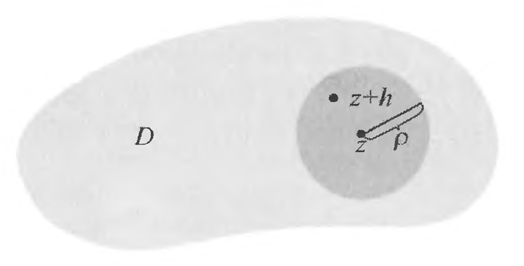
\includegraphics[scale=0.39]{Images/neighborhood.png}
    \caption{The set $U_\rho$}
\end{figure}
Let $f$ be a complex function and $c\in D$. If the limits 
$$
f^\prime(z) =\lim_{h\rightarrow 0} \frac{f\left( z+h \right) -f\left( z \right)}{h}
$$
exists, then $f$ is said to be \textbf{differentiable} at $z$. If $f$ is said to be differentiable if for all $z\in D$ we have $f^\prime(z)$ exists.\par
We now turn to a discussion of the so-called \textbf{Cauchy-Riemann equations}. First note that if $f$ is differentiable, then we may rewrite the definition of differentiable into the following: 
$$
f\left( z+h \right) -f\left( z \right) =f^{\prime}\left( z \right) h+O\left( h \right) ,
$$
where $O(h)$ is a infinitesimal. Now suppose
$$
f\left( z \right) =f\left( x+\mathrm{i}y \right) =f\left( x,y \right) =u\left( x,y \right) +\mathrm{i}v\left( x,y \right) ,
$$
and 
$h=\Delta x+\mathrm{i}\Delta y$, $f^\prime(z)=p+\mathrm{i}q$, $\Delta w=f(z+h)-f(z)=\Delta u+\mathrm{i}\Delta v$, then 
$$
\Delta u+\mathrm{i}\Delta v=\left( p+\mathrm{i}q \right) \left( \Delta x+\mathrm{i}\Delta y \right) +O\left( \sqrt{\Delta ^2x+\Delta ^2y} \right) .
$$
Taking real and imaginary part we obtain 
$$
\Delta u=p\Delta x-q\Delta y+O\left( \sqrt{\Delta ^2x+\Delta ^2y} \right) ,\hspace{0.5cm}\Delta v=p\Delta y+q\Delta x+O\left( \sqrt{\Delta ^2x+\Delta ^2y} \right) .
$$
From this we conclude 
$$
u_x\left( x,y \right) =v_y\left( x,y \right) =p,\hspace{0.5cm}u_y\left( x,y \right) =-v_x\left( x,y \right) =-q.
$$
Therefore if $f$ is differentiable, we have $u$ and $v$ satisfy the following equations: 
\begin{equation}\label{1.2}
\frac{\partial u}{\partial x}=\frac{\partial v}{\partial y},\hspace{0.5cm}\frac{\partial v}{\partial x}=-\frac{\partial u}{\partial y}.
\end{equation}
We call \eqref{1.2} \textbf{Cauchy-Riemann equation}. A trivial observation is if $f$ is differentiable, then 
$$
f^{\prime}\left( z \right) =p+\mathrm{i}q=u_x\left( x,y \right) +\mathrm{i}v_x\left( x,y \right) =v_y\left( x,y \right) -\mathrm{i}u_y\left( x,y \right) .
$$
Conversely, suppose $f(z)=u(x,y)+\mathrm{i}v(x,y)$ with $u$ and $v$ satisfy the Cauchy-Riemann equation, then take 
$$
p=\frac{\partial u}{\partial x}=\frac{\partial v}{\partial y},\hspace{0.5cm}q=-\frac{\partial u}{\partial y}=\frac{\partial v}{\partial x},
$$
we have 
$$
\Delta u=p\Delta x-q\Delta y+O\left( \sqrt{\Delta ^2x+\Delta ^2y} \right) ;\hspace{0.5cm}\Delta v=p\Delta x+q\Delta y+O\left( \sqrt{\Delta ^2x+\Delta ^2y} \right) ,
$$
hence 
$$
f\left( z+h \right) -f\left( z \right) =\Delta u+\mathrm{i}\Delta v=\left( p+\mathrm{i}q \right) \left( \Delta x+\mathrm{i}\Delta y \right) +O\left( \left| h \right| \right) .
$$
Therefore 
$$
\lim_{h\rightarrow 0} \frac{f\left( z+h \right) -f\left( z \right)}{h}=\lim_{h\rightarrow 0} \frac{\left( p+\mathrm{i}q \right) \left( \Delta x+\mathrm{i}\Delta y \right) +O\left( \left| h \right| \right)}{h}=p+\mathrm{i}q,
$$
which implies that $f^\prime(z)$ exists. Therefore we have $f$ is differentiable if and only if $u$ and $v$ satisfy the Cauchy-Riemann equations.\par
We mention that, just as functions of real variables, if $f^\prime(z)=0$ for all $z\in D$, then $f$ is a constant. The proof is easy: consider the Cauchy-Riemann functions, since $f^\prime(z)=0$, then we have $u_x=u_y=0$. Therefore $u$ is a constant of $x$ and $y$. Similarly we have analogous results for $v$ and the proof is finished.\par
We introduce the following definition.
\begin{definition}
Let $D$ be a domain, $f$ a complex function defined on $D$ that is differentiable. If $f^\prime(z)$ is continuous over $D$, then $f$ is said to be \textbf{holomorphic} over $D$, denoted $f\in H(D)$.
\end{definition}
The conventional definition of a holomorphic function does not grant the continuity of $f^\prime(z)$. However, in our text we assume $f^\prime(z)$ to be continuous. Indeed, in modern theories, for instance, manifolds, continuous differentiable functions plays a more greater role than functions that are simply differentiable. Therefore our definition here seems more natural. We shall prove later that our definition here is equivalent to the conventional one, i.e. a complex function that is differentiable always have continuous derivation.\par
The following theorem follows immediately from the preceding discussion.
\begin{theorem}
A complex function $f(z)=f(x+\mathrm{i}y)=u(x,y)+\mathrm{i}v(x,y)$ defined on a domain $D$ is holomorphic if and only if its real part $u(x,y)$ and imaginary part $v(x,y)$ are continuously differentiable and satisfy the Cauchy-Riemann equations.
\end{theorem}
\begin{proof}
Suppose $f\in H(D)$. Then trivially $u$ and $v$ satisfy the Cauchy-Riemann equation. Note further $f^{\prime}\left( z \right) =u_x\left( x,y \right) -\mathrm{i}u_y\left( x,y \right) $ is continuous, we therefore have $u_x$ and $u_y$ are both continuous, hence $u$ is continuously differentiable. Similarly $v$ has analogous results.\par
Conversely, suppose $u$ and $v$ satisfy the Cauchy-Riemann equations. Then $f$ is differentiable. Note further $u$ and $v$ are continuously differentiable, therefore $f^{\prime}\left( z \right) =u_x\left( x,y \right) -\mathrm{i}u_y\left( x,y \right) $ is continuous, which finished the proof.
\end{proof}
Just as functions of a real variable, differentiation has the following properties:
\begin{proposition}
Let $f(z)$ and $g(z)$ be two functions that are differentiable over $D$. Then: 
\begin{enumerate}
    \item Suppose $a_1$ and $a_2$ are constant, then 
    $$
    \frac{\mathrm{d}}{\mathrm{d}z}\left( a_1f\left( z \right) +a_2g\left( z \right) \right) =a_1\frac{\mathrm{d}f\left( z \right)}{\mathrm{d}z}+a_2\frac{\mathrm{d}g\left( z \right)}{\mathrm{d}z};
    $$
    \item 
    $$
    \frac{\mathrm{d}}{\mathrm{d}z}f\left( z \right) g\left( z \right) =\frac{\mathrm{d}f\left( z \right)}{\mathrm{d}z}g\left( z \right) +f\left( z \right) \frac{\mathrm{d}g\left( z \right)}{\mathrm{d}z};
    $$
    \item If $g(z)\ne 0$ over $D$, then 
    $$
    \frac{\mathrm{d}}{\mathrm{d}z}\left( \frac{f\left( z \right)}{g\left( z \right)} \right) =\frac{f^{\prime}\left( z \right) g\left( z \right) -f\left( z \right) g^{\prime}\left( z \right)}{g^2\left( z \right)}.
    $$
\end{enumerate}
\end{proposition}
The proof of the proposition is similar to that of real variables and we omit the details. From this we immediately obtain that the linear combination, product and quotient (provided the denominator is nonzero) of two homomorphic function is also holomorphic. Furthermore, we have the following theorem for the derivative of composite functions.
\begin{theorem}
Let $f$ be a holomorphic function defined on $D$ and $g$ a holomorphic function defined on $E$ such that $f(D)\subset E$. Then $g\circ f$ is also homomorphic and 
$$
\frac{\mathrm{d}}{\mathrm{d}z}f\left( g\left( z \right) \right) =g^{\prime}\left( f\left( z \right) \right) f^{\prime}\left( z \right) .
$$
\end{theorem}
\begin{proof}
Since $f$ and $g$ are both holomorphic, we have 
$$
f\left( z+h \right) -f\left( z \right) =f^{\prime}\left( z \right) h+O\left( h \right) ;\hspace{0.5cm}g\left( w+k \right) -g\left( k \right) =g^{\prime}\left( w \right) k+O\left( k \right) .
$$
Set $w=f\left( z \right) ,k=f\left( z+h \right) -f\left( z \right) $, we have 
$$
\begin{aligned}
g\left( f\left( z+h \right) \right) -g\left( f\left( z \right) \right) &=g^{\prime}\left( f\left( z \right) \right) \left( f\left( z+h \right) -f\left( z \right) \right) +O\left( f\left( z+h \right) -f\left( z \right) \right) 
\\
&=g^{\prime}\left( f\left( z \right) \right) \left( f^{\prime}\left( z \right) h+O\left( h \right) \right) +O\left( f^{\prime}\left( z \right) h+O\left( h \right) \right) 
\\
&=g^{\prime}\left( f\left( z \right) \right) f^{\prime}\left( z \right) h+g^{\prime}\left( f\left( z \right) \right) O\left( h \right) +O\left( f^{\prime}\left( z \right) h+O\left( h \right) \right) 
\\
&=g^{\prime}\left( f\left( z \right) \right) f^{\prime}\left( z \right) h+O\left( h \right) ,
\end{aligned}
$$
therefore 
$$
\frac{\mathrm{d}}{\mathrm{d}z}f\left( g\left( z \right) \right) =\lim_{h\rightarrow 0} \frac{g\left( f\left( z+h \right) \right) -g\left( f\left( z \right) \right)}{h}=g^{\prime}\left( f\left( z \right) \right) f^{\prime}\left( z \right) ,
$$
which finished the proof.
\end{proof}
We use some examples to conclude this section.
\begin{example}\em
We give some examples of holomorphic functions.
\begin{enumerate}
    \item The function $z$ is holomorphic. This is trivial since 
    $$
    \lim_{h\rightarrow 0} \frac{z+h-z}{h}=\lim_{h\rightarrow 0} \frac{h}{h}=1.
    $$
    However, $\bar{z}$ is not holomorphic. Consider 
    \begin{equation}\label{1.3}
    \frac{\overline{z+h}-\overline{z}}{h}=\frac{\bar{z}+\bar{h}-\bar{z}}{h}=\frac{\bar{h}}{h}=\frac{\Delta x-\mathrm{i}\Delta y}{\Delta x+\mathrm{i}\Delta y},
    \end{equation}
    if $\Delta x=0$, then \eqref{1.3} approaches $-1$. However if $\Delta y=0$, then $\eqref{1.3}$ approaches $1$, hence the $\bar{z}$ is not differentiable.
    \item The polynomial 
    \begin{equation}\label{1.4}
    p\left( z \right) =a_0+a_1z+a_2z^2+\cdots +a_nz^n\hspace{0.5cm}\left( a_0,a_1,\cdots ,a_n\in \mathbb{C} \right) 
    \end{equation}
    is holomorphic by the preceding discussion. Note also if $p(z)$ and $q(z)$ are both polynomials, then $p(z)/q(z)$ is also homomorphic excluding the zeros of $q(z)$. It is easy via induction to show that 
    $$
    \frac{\mathrm{d}}{\mathrm{d}z}z^n=nz^{n-1}.\hspace{0.5cm}\left( n\ge 1 \right) 
    $$
    Therefore the derivative of \eqref{1.4} is 
    $$
    \frac{\mathrm{d}p\left( z \right)}{\mathrm{d}z}=a_1+2a_2z+\cdots +na_nz^{n-1}.
    $$
\end{enumerate}
\end{example}
\subsection{Power Series}
